\documentclass[noamssymb]{beamer}
\usepackage[utf8]{inputenc}
\usepackage[english]{babel}
% \usepackage[margin=1in]{geometry}
 % \newcommand\hmmax{0}
% \newcommand\bmmax{0}

% % % Fonts% %
   \usepackage[T1]{fontenc}
   % \usepackage{textcomp}
   % \usepackage{newtxtext}
   % \renewcommand\rmdefault{Pym} %\usepackage{mathptmx} %\usepackage{times}
   \usepackage[complete, subscriptcorrection, slantedGreek, mtpfrak, mtpbbi, mtpcal]{mtpro2}
   \usepackage{bm}% Access to bold math symbols
   \usepackage[no-math]{fontspec}
   \defaultfontfeatures{Ligatures=TeX,Numbers={Proportional}}
   \newfontfeature{Microtype}{protrusion=default;expansion=default;}
   \setmainfont[Ligatures=TeX]{TimesNRMTPro}
   \setsansfont[Scale=MatchLowercase,Ligatures=TeX]{Myriad Pro}
   \setmonofont[Scale=0.8]{mononoki}

   \newfontfamily{\unifont}[Ligatures=TeX]{Menlo}
   \newfontfamily{\ftf}[Ligatures=TeX]{Comic Neue Angular}
   % \usepackage{selnolig}% For suppressing certain typographic ligatures automatically
   \usepackage{microtype}
% % % % % % % % %
% \usepackage{amsthm}         % (in part) For the defined environments
% \usepackage{mathtools}      % Improves  on amsmaths/mtpro2
\usepackage{bbding}         % For hand pointers, etc.

% % The bibliography % % %
\usepackage[backend=biber,
            style=authoryear-comp,
            citestyle=authoryear-comp,
            backref=false,
            % hyperref=true,
            url=false,
            isbn=false,
           ]{biblatex}
% % \renewcommand*{\bibfont}{\small}
% \setlength\bibitemsep{1.5\itemsep}
\addbibresource{ling245.bib}
% \newcommand{\seccite}[1]{\citeauthor{#1}, \citetitle{#1}, \citeyear{#1}}
% % % % % % % % % % % % % % %

% % % % % % % % % % % % % % % % % % % % % % % % % % % % % %

% % % Custom Commands % % %
% \newcommand{\subfor}[2]{[\sfrac{#1}{#2}]}
\usepackage{xfrac,nicefrac} % For \sfrac{i}{j} and for nicer fractions
\newcommand{\sem}[1]{\ensuremath{[\kern-.5mm[{#1}]\kern-.5mm]}}
% % % % % % % % % % % % % %

\usepackage[inline]{enumitem}
% \setlist[enumerate]{itemsep=.03125em}
  \setlist[itemize]{noitemsep}
  % \setlist[description]{noitemsep,style=unboxed,leftmargin=.5cm,font=\normalfont\space}
  \setlist[enumerate]{noitemsep}
% % %

% % For Figures % % %
\usepackage{tikz} % For drawings
\usetikzlibrary{shadows}
\usetikzlibrary{arrows,positioning}
\usepackage{graphicx}
\usepackage{pgfplots}

% \pgfplotsset{compat=1.15}
\usepackage{wrapfig}
\usepackage{float} % For correctly placed floats
\usepackage{subcaption}
% \captionsetup{compatibility=false}
% % % % % % % % % % %

% % % Misc packages % % %

% \usepackage{refcheck} % Can be used for checking references
% \usepackage{lineno}   % For line numbers
% \usepackage{multicol} % For multiple columns
% \usepackage{mathrsfs} % For elegant Latin math letters
% \usepackage{hyphenat} % For \hyp{} hyphenation command, and general hyphenation stuff
% \usepackage{titling} % for multiple titles
% % % % % % % % % % % % %

\usepackage{changepage}
\usepackage[export]{adjustbox}

 \usepackage{pifont}
 \newcommand{\hand}{\ding{43}}

\title{\ftf Ling 245 Project Presentation}
\author{Benjamin Sparkes}
% \date{}

\begin{document}

% % Begin data
\pgfplotstableread[row sep=\\, col sep=&]{
primeCategory  & meanPercent & meanPlusSEPercent& meanMinusSEPercent&  rawMean  &  rawSD   & rawSE & rawMeanPlusSE & rawMeanMinusSE & percentError \\
strongNUM4NUM4 &  0.6767956 & 0.7208479 & 0.6327433 &  2.634409 & 1.653619 & 0.1714723 & 2.805881 & 2.462936 & 0.0511447 \\
weakNUM4NUM4 &  0.5675553 & 0.6129002 & 0.5222103 &  2.184783 & 1.683334 & 0.1745536 & 2.359336 & 2.010229 & 0.0526454 \\
}\NUMNUMData


\pgfplotstableread[row sep=\\, col sep=&]{
primeCategory  & meanPercent & meanPlusSEPercent& meanMinusSEPercent&  rawMean  &  rawSD   & rawSE & rawMeanPlusSE & rawMeanMinusSE & percentError \\
strongNUM4SOME &  0.5762712 & 0.6226379 & 0.5299045 &  2.193548 & 1.702032 & 0.1764925 & 2.370041 & 2.017056 & 0.0538317 \\
weakNUM4SOME &  0.5833029 & 0.6305801 & 0.5360257 &  2.239130 & 1.750162 & 0.1814834 & 2.420614 & 2.057647 & 0.0548888 \\
}\NUMSOMEData

\pgfplotstableread[row sep=\\, col sep=&]{
primeCategory  & meanPercent& meanPlusSEPercent& meanMinusSEPercent&  rawMean  &  rawSD   & rawSE & rawMeanPlusSE & rawMeanMinusSE & percentError \\
strongSOMENUM4 &  0.7414502 & 0.7903533 & 0.6925471 &  2.511364 & 1.597371 & 0.1656396 & 2.677003 & 2.345724 & 0.0567766 \\
weakSOMENUM4 &  0.6498584 & 0.6947576 & 0.6049591 &  2.466667 & 1.643510 & 0.1704240 & 2.637091 & 2.296243 & 0.052128 \\
}\SOMENUMData

\pgfplotstableread[row sep=\\, col sep=&]{
primeCategory  & meanPercent& meanPlusSEPercent& meanMinusSEPercent&  rawMean  &  rawSD   & rawSE & rawMeanPlusSE & rawMeanMinusSE & percentError \\
strongSOMESOME &  0.6966165 & 0.7497500 & 0.6434830 &  2.329545 & 1.713514 & 0.1776831 & 2.507229 & 2.151862 & 0.061688 \\
  weakSOMESOME &  0.4780198 & 0.5732846 & 0.4780198 &  1.978261 & 1.728737 & 0.1792617 & 2.157523 & 1.798999 & 0.1106024 \\
}\SOMESOMEData
% % End data


\begin{frame}
  \maketitle
\end{frame}


\begin{frame}
  \frametitle{{\ftf Motivation}}

  \begin{quote}
    Our approach was to test whether enrichments can be primed across expressions.
    If different sorts of enrichments can prime each other, there must be an abstract mechanism that is shared between them.
    By testing which enrichments prime each other and which don’t, we can specify what the common mechanism might be.\nolinebreak
    \hfill(\citeyear[118]{Bott:2016aa})
\end{quote}

\begin{itemize}
\item[\hand] Are there are shared reasoning processes which apply to distinct instances of enrichment via alternatives, or whether each category of enrichment has its on specialised process?
  \begin{itemize}
  \item[\(\leadsto\)] \citeauthor{Bott:2016aa} are interested in whether priming can occur at all \emph{given} a prior assumption of enrichment via alternatives.
  \end{itemize}
\end{itemize}
\end{frame}

\begin{frame}
  \frametitle{{\ftf Thoughts on the Question}}
 The question of whether or not there are shared reasoning processes which apply to distinct instances of enrichment via alternatives, or whether each category of enrichment has its on specialised process has a nice cognitive feel.

 \begin{itemize}
  \item Intuitively there's some positive upshot whichever way the data points.
    \begin{enumerate}[label=(\roman*)]
    \item If there is cross-category enrichment, then there is a need to posit shared reasonig processes.
    \item If there is no cross-category enrichment, then one should posit distinct reasoning processes.
    \end{enumerate}
    \end{itemize}
  However, it is important to note that each of these carries a presupposition that the data can/should/will support one of these resolutions.

\end{frame}

\begin{frame}
  \frametitle{{\ftf \citeauthor{Bott:2016aa}'s Experiments}}

  \citeauthor{Bott:2016aa} ran three experiments.

  Participants were presented with trials consisting of a setence and two picutures, and are asked to select the picture which best reflects the sentence.

  Trials are split into \emph{prime} and \emph{response}.
  \begin{itemize}
  \item Prime and response trials have the same structure.
  \item Every response trial is preceeded by two prime trials.
  \item Prime trials are used to ensure the participant considers certain alternatives.
  \end{itemize}


\end{frame}

\begin{frame}
  \frametitle{{\ftf \citeauthor{Bott:2016aa}'s Experiments}}
  \begin{itemize}
  \item Prime trials:
    \begin{itemize}
    \item \emph{Weak}: One false picture, and one true but underinformative picture.
    \item \emph{Strong}: Two true pictues. One true informative picture, the other underinformative.
    \end{itemize}
  \item Response trials:
    \begin{itemize}
    \item One picture true but underinformative picture.
    \item A picture containg the words `Better Picture?'
    \end{itemize}
  \item[\hand] Participants were instructed to click the `Better Picture?' option  if they felt the the other picture did not sufficiently capture the sentence meaning.
  \end{itemize}
\end{frame}



\begin{frame}
  \frametitle{{\ftf Details of the Experiment}}

The sentences were constructed using one of two frames:
\begin{enumerate}[label=(\roman*)]
\item Some of the symbols are [symbol]
\item There are four [symbol]
\end{enumerate}

\citeauthor{Bott:2016aa} included a third frame:
\begin{enumerate}[label=(\roman*), resume]
\item There is a [symbol].
\end{enumerate}

The symbols were randomly chosen from:
\begin{itemize}
\item  {\space\unifont ♦\space} \mbox{ }  {\space\unifont ♣\space} \mbox{ } {\space\unifont ✓\space} \mbox{ } {\space\unifont ♠\space} \mbox{ } {\space\unifont ♥\space} \mbox{ } {\space\unifont ◼\space} \mbox{ } {\space\unifont ★\space} \mbox{ } {\space\unifont ●\space} \mbox{ } {\space\unifont ♩\space} \mbox{ } {\space\unifont ▲}
\end{itemize}
Sentences and pictures were generated for each participant at the start of each experiment.

Four instances of each prime strength, prime category, and reponse category combination were included in the trial.
\end{frame}

\begin{frame}
  \frametitle{{\ftf Example}}

  \begin{adjustbox}{width=1.3\textwidth, center=13cm}
  \begin{tikzpicture}
    \draw (-7,0) -- (-2,0);
    \node[text width=6cm] at (-2,5) {\emph{Prime}};
    \node[text width=6cm] at (7,5) {\emph{Target}};
    \node[text width=6cm] at (-5.75,2.125) {\emph{Strong}};
    \node[text width=6cm] at (-5.75,-2.375) {\emph{Weak}};
    \node[text width=6cm] at (-3.9,4) {\textsf{Some of the symbols are squares}};
    \node[inner sep=0pt] (p1L) at (-6,2) {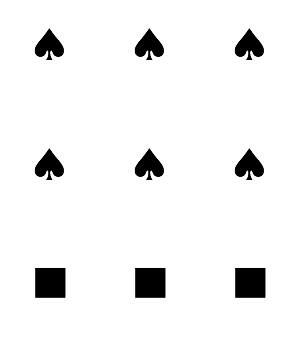
\includegraphics[width=.15\linewidth, fbox]{images/p1LSpquares.png}};
    \node[inner sep=0pt] (p1R) at (-3,2) {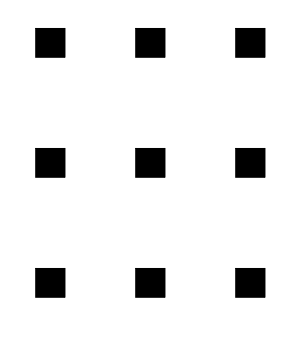
\includegraphics[width=.15\linewidth, fbox]{images/p1RSquares.png}};
    \node[text width=6cm] at (-3.8,-.5) {\textsf{Some of the symbols are stars}};
    \node[inner sep=0pt] (p2L) at (-6,-2.5) {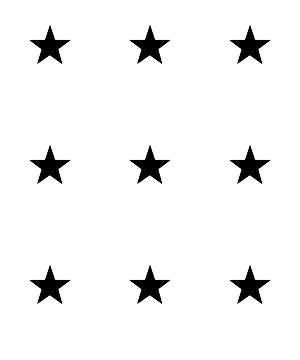
\includegraphics[width=.15\linewidth, fbox]{images/p2LStars.png}};
    \node[inner sep=0pt] (p2R) at (-3,-2.5) {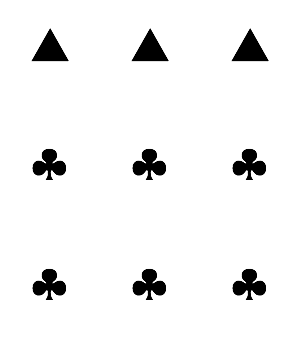
\includegraphics[width=.15\linewidth, fbox]{images/p2RStars.png}};
    \node[text width=6cm] at (5.375,2) {\textsf{Four of the symbols are hearts}};
    \node[inner sep=0pt] (rL) at (3,0) {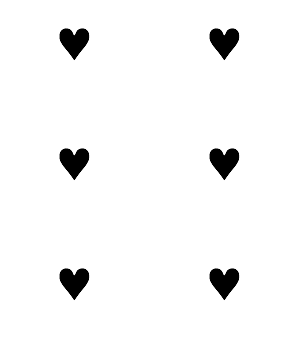
\includegraphics[width=.15\linewidth, fbox]{images/responseFourH.png}};
    \node[inner sep=0pt] (rR) at (6,0) {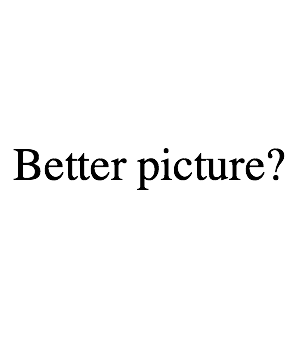
\includegraphics[width=.15\linewidth, fbox]{images/bp.png}};
    \draw[->] (-1,2) -- (.75,1);
    \draw[->] (-1,-2) -- (.75,-1);
  \end{tikzpicture}
\end{adjustbox}


\end{frame}

\begin{frame}
  \frametitle{{\ftf `Correct' Responses}}

  For each prime trials there was a `correct' response, either due to the semantic content of the sentence in the case of weak trials, or due to pragmatics in the case of strong trials.
  \begin{quote}
    [I]n the presence of both a weak picture and a strong picture, participants could not make a non-arbitrary choice solely based on the truth conditions of the weak interpretation which is true in both cases, hence the strong reading is a favored option in that it provides a non-arbitrary way to resolve the task.\nolinebreak
    \hfill(\citeyear[124]{Bott:2016aa})
  \end{quote}


  Linking hypothesis:
  \begin{itemize}
  \item[\hand] Prior trials will effect how participants evaluate sentences, and that in response trials participants click on `Better Picture?' if they process the setence pragmatically, and the semantically adequate picture otherwise.
  \end{itemize}
\end{frame}

\begin{frame}
  \frametitle{{\ftf Picture Details}}

  \begin{itemize}
  \item \emph{Some} trials:
    \begin{itemize}
    \item \textbf{Strong pictures}: involved three symbols matching the predicate in the sentence, and six of another type.
    \item \textbf{Weak pictures}: Nine symbols matching the predicate in the sentence.
    \item \textbf{False pictures}: Nine symbols of the same type which did not match the predicate.
    \end{itemize}

    \item \emph{Number}4 trials:
    \begin{itemize}
    \item \textbf{Strong pictures}: Symbols matching the number and predicate in the sentence, the number was always `four'.
    \item \textbf{Weak pictures}:  A greater number of symbols than in the sentence which matched the predicate, this was always six.
    \item \textbf{False pictures}: A smaller number of symbols than in the sentence which matched the predicate, this was always two.
    \end{itemize}
  \end{itemize}

\end{frame}



\begin{frame}
  \frametitle{{\ftf Filler Trials}}

  Filler trials were also included:

  \begin{itemize}
  \item \emph{All} sentences, an alternative to \emph{some}.
  \item \emph{Number}6 sentences, an alternative to \emph{number}4.
  \end{itemize}

Each could occur in three forms:
\begin{enumerate}[label=(\arabic*)]
\item a weak picture with symbols that did not match the predicate in the sentence, and a ``Better Picture?'' option
\item a weak picture with symbols that matched the predicate, and a ``Better Picture?'' option, and
\item a weak picture with symbols that matched the predicate, and a strong picture.
\end{enumerate}
\citeauthor{Bott:2016aa} used these to highlight alternatives to participants.
One filler triplet every six target triplets.
\end{frame}


\begin{frame}
  \frametitle{{\ftf The `Replication'}}
  Partial replication for two reasons:
\begin{enumerate}[label=\arabic*)]
\item Half the number of participants compared with the original experiment (100 and 200 participants, respectively)
\item Only two enrichment categories, as opposed to three in the original.
\item We included keyboard shortcuts
\item Areas where \citeauthor{Bott:2016aa} weren't super clear on details
\end{enumerate}
The basis for both modifications were straightforward cost considerations.

By uncommenting a few lines of code (and fixing any bugs that this may cause) the full experiment can be run.

{\footnotesize
\texttt{https://github.com/bsparkes/bottchemla2016}
\texttt{https://bsparkes.github.io/bottchemla2016/experiment/html/bottchemla2016.html}
}

\end{frame}


\begin{frame}
\frametitle{{\ftf Predictions}}

\citeauthor{Bott:2016aa} did not make predictions regarding the results of the experiment.
\begin{itemize}
\item[\(\leadsto\)] Core interest is in how the question about EVAs should be resolved.
\end{itemize}


They do note:
\begin{quote}
  If enrichment can be primed at all, we would expect within-category priming \dots [and] \dots If the \emph{numbers}, \emph{some} and \emph{ad hoc} EVAs share enrichment mechanisms we would expect them to prime each other, so that a strong some prime, for example, leads to a greater proportion of strong number responses.\linebreak
  \mbox{ }\hfill(\citeyear[122]{Bott:2016aa})
\end{quote}

From the results of \citeauthor{Bott:2016aa}'s experiment, one would expect to see a significant effect of priming, both within and between categories.
\end{frame}

\begin{frame}

  \frametitle{{\ftf Results}}

  \begin{enumerate}[label=\arabic*.]
  \item Significant replication of priming effects in general.
  \item Almost significant replication of within category priming effect.
  \item Failure to replicate between category priming effect.
  \item Different kinds of priming effects, for within category priming.
  \item Replication of no significant effects when splitting the data in half.
  \end{enumerate}

  \begin{itemize}
  \item[\hand] Less support for shared reasoning processes between distinct instances of enrichment via alternatives?
  \end{itemize}

\end{frame}


\begin{frame}

  \frametitle{{\ftf A Bar Plot}}

  \begin{adjustwidth}{-1em}{-0em}
    \begin{figure}[ht]
      \begin{subfigure}[]{.25\textwidth}
        \begin{tikzpicture}
          \begin{axis}[
            align =center,
            title = {Num4 \\ Num4},
            width=4cm,
            height=8cm,
            ybar=2*\pgflinewidth,
            enlarge x limits=1,
            bar width=25pt,
            symbolic x coords={strongNUM4NUM4, weakNUM4NUM4},
            xticklabels = {Strong, Weak},
            xtick={strongNUM4NUM4, weakNUM4NUM4},
            grid=major,
            ymax=1,
            ymin=0,
            enlarge x limits=.75,
            ]
            \addplot+[error bars/.cd,y dir=both,y explicit] table[x=primeCategory,y=meanPercent, y error=percentError]{\NUMNUMData};
          \end{axis}
        \end{tikzpicture}
      \end{subfigure}\hfill
      \begin{subfigure}[]{.25\textwidth}
        \begin{tikzpicture}
          \begin{axis}[
            align =center,
            title = {Num4 \\ Some},
            width=4cm,
            height=8cm,
            ybar=2*\pgflinewidth,
            enlarge x limits=1,
            bar width=25pt,
            symbolic x coords={strongNUM4SOME, weakNUM4SOME},
            xticklabels = {Strong, Weak},
            xtick={strongNUM4SOME, weakNUM4SOME},
            grid=major,
            ymax=1,
            ymin=0,
            yticklabels=\empty,
            enlarge x limits=.75,
            ]
            \addplot+[error bars/.cd,y dir=both,y explicit] table[x=primeCategory,y=meanPercent, y error=percentError]{\NUMSOMEData};
          \end{axis}
        \end{tikzpicture}
      \end{subfigure}%\hspace{2pt}
      \begin{subfigure}[]{.25\textwidth}
        \begin{tikzpicture}
          \begin{axis}[
            align =center,
            title = {Some \\ Num4},
            width=4cm,
            height=8cm,
            ybar=2*\pgflinewidth,
            enlarge x limits=1,
            bar width=25pt,
            symbolic x coords={strongSOMENUM4, weakSOMENUM4},
            xticklabels = {Strong, Weak},
            xtick={strongSOMENUM4, weakSOMENUM4},
            grid=major,
            ymax=1,
            ymin=0,
            yticklabels=\empty,
            enlarge x limits=.75,
            ]
            \addplot+[error bars/.cd,y dir=both,y explicit] table[x=primeCategory,y=meanPercent, y error=percentError]{\SOMENUMData};
          \end{axis}
        \end{tikzpicture}
      \end{subfigure}%\hspace{pt}
      \begin{subfigure}[]{.25\textwidth}
        \begin{tikzpicture}
          \begin{axis}[
            align =center,
            title = {Some \\ Some},
            width=4cm,
            height=8cm,
            ybar=2*\pgflinewidth,
            enlarge x limits=1,
            bar width=25pt,
            symbolic x coords={strongSOMESOME, weakSOMESOME},
            xticklabels = {Strong, Weak},
            xtick=data,
            grid=major,
            ymax=1,
            ymin=0,
            yticklabels=\empty,
            enlarge x limits=.75,
            ]
            \addplot+[error bars/.cd,y dir=both,y explicit] table[x=primeCategory,y=meanPercent, y error=percentError]{\SOMESOMEData};
          \end{axis}
        \end{tikzpicture}
      \end{subfigure}
    \end{figure}
  \end{adjustwidth}
\end{frame}

\begin{frame}
  \frametitle{{\ftf Data Treatment}}


\citeauthor{Bott:2016aa} use the fact that each target trial was preceded by two prime trials this design to filter out target responses where they cannot be sure that the participant understood the correct interpretation of the prime sentence.

In terms of a comparison of relative target response removals, the numbers are 6.5\% (B\&C) and 7.1\% (R) of all trials.

As \citeauthor{Bott:2016aa} do not include information about the categories the incorrect primes were removed from, so we don't have sufficient information to provide further insights.

\end{frame}

\begin{frame}
  \frametitle{{\ftf Data Treatment}}

One hundred participants were recruited using Amazon Turk.
\begin{itemize}
\item We removed 7 participants who did not declare English as their native language.
\end{itemize}


We included keyboard shortcuts to help participants complete the experiment.

This  meant that in principle the participants could complete the experiment very quickly.
\begin{itemize}
\item E.g., going through the experiment as fast as possible (using the keyboard, not reading the sentnces, etc.) takes around 40 seconds.
\end{itemize}
One and a half second seems a reasonable lower bound for time spent on a trail.
\begin{itemize}
\item 3 mins lower bound, average time of 9 mins.
\end{itemize}
  One participant who feel below this, after the lang.\ restrictions.

\end{frame}



\begin{frame}
  \frametitle{{\ftf Analysis Procedure}}

  Following \citeauthor{Bott:2016aa} the response-type likelihood was modelled using logit mixed-effect models.

  Analyses were conducted lme4 (\cite{Bates:2014aa}), languageR (\cite{Baayen:2011aa}), and memisc (\cite{Elff:2012aa}), libraries for the R statistics program (\cite{Team:2013aa}).

  Treatment and sum coding were used as described by \citeauthor{Bott:2016aa}, with any factor not explicitly mentioned receiving treatment contrasts.

  The analysis starts with an general model involving all of the data, in which the interaction of with and between-expression priming is assessed.

  A more detailed analysis is then performed by restricting the analysis to within and between-expression trials only.

  The dependent measure was the log odds of choosing a strong over a weak prime.

\end{frame}



\begin{frame}

  \frametitle{{\ftf Analysis}}

  \citeauthor{Bott:2016aa} report three analyses:

  \begin{enumerate}[label=\arabic*.]
  \item Whether EVAs can be primed at all,
  \item Whether priming occurs at the within-category level, and
  \item Whether priming occurs at the between-category level.
  \end{enumerate}

\end{frame}

\begin{frame}
  \frametitle{{\ftf Without the \(\beta\)s, Avoiding the \emph{p}s, and Forgetting the \emph{Z}s}}

  \citeauthor{Bott:2016aa} observed priming of EVAs at the within-category level and the between category level, we only observed priming of EVAs at the within-category level.
\end{frame}


\begin{frame}

  \frametitle{{\ftf Fancy Results: Overview}}

  \citeauthor{Bott:2016aa}:
    \begin{adjustbox}{width=1\textwidth,center=\textwidth}
    \begin{tabular}{llrrrr}
      \hline
      & & \(\beta\) & S.E.\ & \emph{Z} & \emph{p}-value  \\
      \hline
      Overview & \(\text{Prime} * \text{WithBet} + (1 + \text{Prime} * \text{WithBet} \mid \text{subject})\) & & & \\
      & (Intercept) & \(-\)0.594 & 0.198 & \(-\)2.991 & .003 \\
      & Prime & 0.563 & 0.034 & 16.342 & <.001 \\
      & WithBet & 0.126 & 0.029 & 4.284 & <.001 \\
      & Prime:WithBet & \(-\)0.430 & 0.033 & \(-\)13.177 & <.001 \\
      Within simple & Prime & 0.993 & 0.059 & 16.950 & <.001 \\
      Between Simple & Prime & 0.133 & 0.033 & 4.082 & <.001 \\
      \hline
    \end{tabular}
  \end{adjustbox}

Replication:
\begin{adjustbox}{width=1\textwidth,center=\textwidth}
    \begin{tabular}{llrrrr}
      \hline
      & & \(\beta\) & S.E.\ & \emph{Z} & \emph{p}-value  \\
      \hline
      Overview & \(\text{Prime} * \text{WithBet} + (1 + \text{Prime} * \text{WithBet} \mid \text{subject})\) & & & \\
      & (Intercept)   & 0.962  & 0.346 &  2.778 & <.010 \\
      & Prime         & 0.310  & 0.074 &  4.196 & <.001 \\
      & WithBet       & \(-\)0.006 & 0.067 & \(-\)0.089 &  .929 \\
      & Prime:WithBet & 0.294  & 0.071 &  4.135 & <.001 \\
      Between Simple & Prime & 0.016 & 0.089 & 0.181 & .857  \\
      Within Simple  & Prime & 0.603 & 0.114 & 5.277 & <.001 \\
      \hline
    \end{tabular}
  \end{adjustbox}

\end{frame}

\begin{frame}
  \frametitle{{\ftf Details}}

  For the first model, sum contrasts are used for both factors, and a significant effect of a strong prime increasing the rate of strong responses, \(\beta = 0.56\), \emph{p} \(< .001\), a significant effect of strong responses happening in between category trials, rather than within category, \(\beta = 0.126\), \emph{p} \(< .001\) and an interaction between the two \(\beta = -0.43\), \emph{p} \(< .001\) showing that the effect of the prime was greater in between within trials.

We observed slightly different results.
First, a significant effect of priming \(\beta = 0.310\), \emph{p} \(<.001\) for within category trials, no significant effect of between category trials, \emph{p} \(= .929\), but a significant effect of the interaction between the two \(\beta = .294\), \emph{p} \(<.001\).
So, the effect of prime was less for between category trails.
Though, in all cases these effects were smaller than those observed by \citeauthor{Bott:2016aa}.
\end{frame}

\begin{frame}
  \frametitle{{\ftf Simple Effects}}
  \citeauthor{Bott:2016aa} use a model with a similar structure, but using treatment contrasts for the within/between factor and sum contrasts for the prime factor to investigate simple effects.

  They observe significant priming occurred at the within category level, \(\beta = .99\), \emph{p} \(< .001\), and at the between category level \(\beta = .13\), \emph{p} \(< .001\).

  We observe significant priming at the within category level \(\beta = .603\), \emph{p} \(<.001\), but no significant priming at the between category level \(\beta = .016\), \emph{p} \(< .857\).

  Now, I don't really understand all the details here, but from what I gather this means the effect of between category priming is significant \emph{given} the effect of within category priming, but not really significant in and of itself.

\end{frame}


\begin{frame}
  \frametitle{{\ftf Details: Further Observations}}

  \citeauthor{Bott:2016aa} broke the data down into within-category trials and between-category trials to assess the observed effects in more detail, conducting separate analyses on each.
  In each model treatment contrasts were used for the categories, and sum contrasts for the prime.

\end{frame}


\begin{frame}
  \frametitle{{\ftf Details: Within}}
  \citeauthor{Bott:2016aa} observed a significant effect of prime, \(\beta = 1.24\), \emph{p} \(< .001\), for within category trials, showing an effect for \emph{ad hoc} categories.
  In contrast to \citeauthor{Bott:2016aa} we found a significant effect for the \emph{number}4 category, \(\beta = 0.759\), \emph{p} \(< .001\).
  And, in line with \citeauthor{Bott:2016aa}, we did not find a significant effect with respect for the \emph{some} category.

\end{frame}

\begin{frame}

  \frametitle{{\ftf Fancy Results: Within}}

  \citeauthor{Bott:2016aa}:
    \begin{adjustbox}{width=1\textwidth,center=\textwidth}
    \begin{tabular}{llrrrr}
      \hline
      & & \(\beta\) & S.E.\ & \emph{Z} & \emph{p}-value  \\
      \hline
      Within detail & \multicolumn{2}{l}{\(\text{Prime} * \text{WithCat} + (1 + \text{Prime} * \text{WithCat} \mid \text{subject})\)}  & & & \\
      & (Intercept)  & \(-\)2.088 & 0.255 & \(-\)8.185 & <.001\\
      & Prime & 1.239 & 0.109 & 11.374 & <.001 \\
      & WithCatNUM4 & 2.068 & 0.195 & 10.588 & <.001 \\
      & WithCatSOME & 1.823 & 0.157 & 11.598 & <.001 \\
      & Prime:WithCatNUM4 & 0.174 & 0.166 & 1.046 & .269 \\
      & Prime:WithCatSOME & \(-\)0.138 & 0.137 & \(-\)1.007 & .314 \\

      \hline
    \end{tabular}
  \end{adjustbox}
Replication:
\begin{adjustbox}{width=1\textwidth,center=\textwidth}
    \begin{tabular}{llrrrr}
      \hline
      & & \(\beta\) & S.E.\ & \emph{Z} & \emph{p}-value  \\
      \hline
      Within Detail & \multicolumn{2}{l}{\(\text{Prime} * \text{WithCat} + (1 + \text{Prime} * \text{WithCat} \mid \text{subject})\)}  & & & \\
      & (Intercept)   &  1.361 & 0.460 &  2.960 & <.010 \\
      & Prime         &  0.759 & 0.206 &  3.678 & <.001 \\
      & WithCatSOME       & \(-\)0.784 & 0.432 & \(-\)1.816 & .069  \\
      & Prime:WithCatSOME & \(-\)0.164 & 0.265 & \(-\)0.618 & .536  \\
      \hline
    \end{tabular}
  \end{adjustbox}

\end{frame}


\begin{frame}
  \frametitle{{\ftf Details: Between}}

  Between categories, \citeauthor{Bott:2016aa} found a significant effect of priming \(\beta = .15\), \emph{p} \(< .05\) for \emph{number}4/\emph{ad hoc} trials and for \emph{some}/\emph{number}4 trials, but not when interaction with the strength of the prime was accounted for, and we found no significant interaction.

  \citeauthor{Bott:2016aa} also perform further analysis of the data pooled from three experiments they conducted.

  We followed a similar analysis, looking at the separate prime and target categories in the case of between category trials and with splits of the data into first and second halves of the experiment.

  In contrast to \citeauthor{Bott:2016aa} analysing the separate prime and target categories in the case of between category trials revealed no significant effects, and in line with \citeauthor{Bott:2016aa} the split by halves did not reveal a difference in responses.

\end{frame}

\begin{frame}

  \frametitle{{\ftf Fancy Results: Between}}
  \citeauthor{Bott:2016aa} (directions pooled):
  \begin{adjustbox}{width=1\textwidth,center=\textwidth}
    \begin{tabular}{llrrrr}
      \hline
      & & \(\beta\) & S.E.\ & \emph{Z} & \emph{p}-value  \\
      \hline
      Between detail & \multicolumn{2}{l}{\(\text{Prime} * \text{BetCat} + (1 + \text{Prime} * \text{BetCat} \mid \text{subject})\)}  & & & \\
      & (Intercept)  & \(-\)0.691 & 0.204 & \(-\)3.384 & <.001\\
      & Prime & 0.145 & 0.058 & 0.058 & .012 \\
      & BetCatSOMEADH & \(-\)0.054 & 0.089 & \(-\)0.611 & .540 \\
      & BetCatSOMENUM4 & 0.889 & 0.112 & 7.915 & <.001 \\
      & Prime:BetCatSOMEADH & \(-\)0.069 & 0.079 & \(-\)0.873 & .383 \\
      & Prime:BetCatSOMENUM4 & 0.078 & 0.088 & 0.888 & .374 \\
      \hline
    \end{tabular}
  \end{adjustbox}

  Replciation (directions \emph{not} pooled):
\begin{adjustbox}{width=1\textwidth,center=\textwidth}
    \begin{tabular}{llrrrr}
      \hline
      & & \(\beta\) & S.E.\ & \emph{Z} & \emph{p}-value  \\
      \hline
      Between detail & \multicolumn{2}{l}{\(\text{Prime} * \text{BetCat} + (1 + \text{Prime} * \text{BetCat} \mid \text{subject})\)}  & & & \\
      & (Intercept)  &  0.899 & 0.506 &  1.777 & .076 \\
      & Prime        & \(-\)0.086 & 0.160 & \(-\)0.541 & .589 \\
      & BetCatSOMENUM4 & 0.861  & 0.451 &  1.910 & .056 \\
      & Prime:BetCatSOMENUM4 &  0.362 & 0.282 &  1.281 & .200 \\
      \hline
    \end{tabular}
  \end{adjustbox}

\end{frame}

\begin{frame}

  \frametitle{{\ftf Analysis of priming effect for direction between category trials}}

  \citeauthor{Bott:2016aa}:
\begin{adjustbox}{width=1\textwidth,center=\textwidth}
    \begin{tabular}{llrrrr}
      \hline
      & & \(\beta\) & S.E.\ & \emph{Z} & \emph{p}-value  \\
      \hline
      & \multicolumn{2}{l}{\(\text{Prime} + (1 + \text{Prime} \mid \text{Subject})\)} & & & \\
      \emph{some} \(\rightarrow\) \emph{number}4 & Prime & 0.345 &  0.069 & 5.140 & <.001 \\
      \emph{number}4 \(\rightarrow\) \emph{some} & Prime & 0.221  & 0.065 & 3.412  & <.001 \\
      \hline
    \end{tabular}
  \end{adjustbox}

  Replciation:
  \begin{adjustbox}{width=1\textwidth,center=\textwidth}
    \begin{tabular}{llrrrr}
      \hline
      & & \(\beta\) & S.E.\ & \emph{Z} & \emph{p}-value  \\
      \hline
      & \multicolumn{2}{l}{\(\text{Prime} + (1 + \text{Prime} \mid \text{Subject})\)} & & & \\
      \emph{some} \(\rightarrow\) \emph{number}4 & Prime & \(-\)0.080 &  0.162 & \(-\)0.492 & 0.623 \\
      \emph{number}4 \(\rightarrow\) \emph{some} & Prime & 0.354  &  0.238 & 1.488  & 0.137 \\
      \hline
    \end{tabular}
  \end{adjustbox}
\end{frame}


\begin{frame}
  \frametitle{{\ftf Observations}}

  So, the motivation was to see what kind of priming processes there were, and whether these were distinct or shared.
  And, from the data gathered, \citeauthor{Bott:2016aa} argue that enrichment can be primed.

  They note that the between-category priming effect illustrates that there are shared mechanisms across the EVA categories.
  However, the greater within-category priming results demonstrate that there are also some additional effect of EVA specific mechanisms.

  I'm no sure that this was replicated.
\end{frame}

\begin{frame}
  \frametitle{{\ftf Observations}}
  We observed that there was a quite different effect of priming for within category trials for \emph{some} and \emph{number}4.
  This is not in line with what \citeauthor{Bott:2016aa} observed.

  For between category trials we didn't have a sufficient number of categories to do the same analysis as \citeauthor{Bott:2016aa} did.
  However, we did observe that there was quite an effect on which categories the prime and target came from.

  As \citeauthor{Bott:2016aa} argue that there's a shared priming process between \emph{some} and \emph{number}4, it doesn't seem that our data supports this.
  For, we should expect that effects would be similar in both directions.

  We have close to significant results for the within category case, but not for the betweeen category case.

\end{frame}


\begin{frame}
  \frametitle{{\ftf Summary}}

  \citeauthor{Bott:2016aa}'s goal  was to better understand how people use alternatives to enrich the basic meaning of a sentence.

  Significant effects of priming both within and between categories were observed, and in particular between \emph{some} and \emph{number}4 categories.

  In our replication we found significant effects of priming within categories, but no significant effects of priming between categories, even when the prime and target categories were controlled for.

  Unclear to me exactly what this means.

\end{frame}


\appendix


\begin{frame}
  \frametitle{{\ftf Don't Go Past This Slide \dots}}

  Additional details follow \dots
\end{frame}


\begin{frame}

  \frametitle{{\ftf Combined Results from \citeauthor{Bott:2016aa}}}

    \begin{adjustbox}{width=1\textwidth,center=\textwidth}
    \begin{tabular}{llrrrr}
      \hline
      & & \(\beta\) & S.E.\ & \emph{Z} & \emph{p}-value  \\
      \hline
      Overview & \(\text{Prime} * \text{WithBet} + (1 + \text{Prime} * \text{WithBet} \mid \text{subject})\) & & & \\
      & (Intercept) & \(-\)0.594 & 0.198 & \(-\)2.991 & .003 \\
      & Prime & 0.563 & 0.034 & 16.342 & <.001 \\
      & WithBet & 0.126 & 0.029 & 4.284 & <.001 \\
      & Prime:WithBet & \(-\)0.430 & 0.033 & \(-\)13.177 & <.001 \\
      Within simple & Prime & 0.993 & 0.059 & 16.950 & <.001 \\
      Between Simple & Prime & 0.133 & 0.033 & 4.082 & <.001 \\
      Within detail & \multicolumn{2}{l}{\(\text{Prime} * \text{WithCat} + (1 + \text{Prime} * \text{WithCat} \mid \text{subject})\)}  & & & \\
      & (Intercept)  & \(-\)2.088 & 0.255 & \(-\)8.185 & <.001\\
      & Prime & 1.239 & 0.109 & 11.374 & <.001 \\
      & WithCatNUM4 & 2.068 & 0.195 & 10.588 & <.001 \\
      & WithCatSOME & 1.823 & 0.157 & 11.598 & <.001 \\
      & Prime:WithCatNUM4 & 0.174 & 0.166 & 1.046 & .269 \\
      & Prime:WithCatSOME & \(-\)0.138 & 0.137 & \(-\)1.007 & .314 \\
      Between detail & \multicolumn{2}{l}{\(\text{Prime} * \text{BetCat} + (1 + \text{Prime} * \text{BetCat} \mid \text{subject})\)}  & & & \\
      & (Intercept)  & \(-\)0.691 & 0.204 & \(-\)3.384 & <.001\\
      & Prime & 0.145 & 0.058 & 0.058 & .012 \\
      & BetCatSOMEADH & \(-\)0.054 & 0.089 & \(-\)0.611 & .540 \\
      & BetCatSOMENUM4 & 0.889 & 0.112 & 7.915 & <.001 \\
      & Prime:BetCatSOMEADH & \(-\)0.069 & 0.079 & \(-\)0.873 & .383 \\
      & Prime:BetCatSOMENUM4 & 0.078 & 0.088 & 0.888 & .374 \\
      \hline
    \end{tabular}
  \end{adjustbox}

\end{frame}

\begin{frame}

\frametitle{{\ftf Combined Results from the Replication}}

\begin{adjustbox}{width=1\textwidth,center=\textwidth}
    \begin{tabular}{llrrrr}
      \hline
      & & \(\beta\) & S.E.\ & \emph{Z} & \emph{p}-value  \\
      \hline
      Overview & \(\text{Prime} * \text{WithBet} + (1 + \text{Prime} * \text{WithBet} \mid \text{subject})\) & & & \\
      & (Intercept)   & 0.962  & 0.346 &  2.778 & <.010 \\
      & Prime         & 0.310  & 0.074 &  4.196 & <.001 \\
      & WithBet       & \(-\)0.006 & 0.067 & \(-\)0.089 &  .929 \\
      & Prime:WithBet & 0.294  & 0.071 &  4.135 & <.001 \\
      Between Simple & Prime & 0.016 & 0.089 & 0.181 & .857  \\
      Within Simple  & Prime & 0.603 & 0.114 & 5.277 & <.001 \\
      Within Detail & \multicolumn{2}{l}{\(\text{Prime} * \text{WithCat} + (1 + \text{Prime} * \text{WithCat} \mid \text{subject})\)}  & & & \\
      & (Intercept)   &  1.361 & 0.460 &  2.960 & <.010 \\
      & Prime         &  0.759 & 0.206 &  3.678 & <.001 \\
      & WithCat       & \(-\)0.784 & 0.432 & \(-\)1.816 & .069  \\
      & Prime:WithCat & \(-\)0.164 & 0.265 & \(-\)0.618 & .536  \\
      Between detail & \multicolumn{2}{l}{\(\text{Prime} * \text{BetCat} + (1 + \text{Prime} * \text{BetCat} \mid \text{subject})\)}  & & & \\
      & (Intercept)  &  0.899 & 0.506 &  1.777 & .076 \\
      & Prime        & \(-\)0.086 & 0.160 & \(-\)0.541 & .589 \\
      & BetCat       & 0.861  & 0.451 &  1.910 & .056 \\
      & Prime:BetCat &  0.362 & 0.282 &  1.281 & .200 \\
      \hline
    \end{tabular}
  \end{adjustbox}

\end{frame}


\begin{frame}
  \frametitle{{\ftf Details for the bar plots}}

\begin{adjustbox}{width=1\textwidth,center=\textwidth}
    \begin{tabular}{rrrrrrrrrr}
      \hline
      \multicolumn{2}{c}{Prime} & Response & \multicolumn{4}{c}{From the replication} & \multicolumn{2}{c}{From Bott and Chelma} \\
      \cline{1-3}
      Type & Category & Category  & mean \% & Raw mean & Raw S.D.\ & Raw S.E.\ &  mean \%  & Raw S.E.\  \\
      \hline
      Strong & Num4 &  Num4 &   0.6767956 &  2.634409 & 1.653619 & 0.1714723  & 0.615 & 0.018   \\
      Weak & Num4 &  Num4 &   0.5675553 &  2.184783 & 1.683334 & 0.1745536  & 0.339 & 0.018    \\
      Strong & Num4 &  Some &   0.5762712 &  2.193548 & 1.702032 & 0.1764925  & 0.553 & 0.019    \\
      Weak & Num4 &  Some &   0.5833029 &  2.239130 & 1.750162 & 0.1814834  & 0.484 & 0.019    \\
      Strong & Some &  Num4 &   0.7414502 &  2.511364 & 1.597371 & 0.1656396  & 0.544 & 0.020    \\
      Weak & Some &  Num4 &   0.6498584 &  2.466667 & 1.643510 & 0.1704240  & 0.474 & 0.019    \\
      Strong & Some &  Some &   0.6966165 &  2.329545 & 1.713514 & 0.1776831  & 0.604 & 0.019    \\
      Weak & Some &  Some &   0.4703510 &  1.978261 & 1.728737 & 0.1792617 & 0.340 & 0.018     \\
      \hline
    \end{tabular}
  \end{adjustbox}

  Relevant cell mean and S.E.\ from \citeauthor{Bott:2016aa} included.
\end{frame}






\begin{frame}
  \frametitle{{\ftf Analysis of the experiment by halves}}

  \begin{adjustbox}{width=1\textwidth,center=\textwidth}
    \begin{tabular}{llrrrr}
      \hline
      & & \(\beta\) & S.E.\ & \emph{Z} & \emph{p}-value  \\
      \hline
      Within by half & \multicolumn{5}{l}{\(\text{Prime} * \text{WithCat} * \text{Half} + (1 + \text{Prime} * \text{WithCat} * \text{Half} \mid \text{Subject})\)}  \\
      & (Intercept)        & \(-\)0.221 & 0.378 & \(-\)0.584 & .559 \\
      & Prime              &  0.141 & 0.320 &  0.442 & .658 \\
      & WithCat            &  1.068 & 0.481 &  2.222 & <.050 \\
      & Half               &  0.850 & 0.371 &  2.294 & <.050 \\
      & Prime:WithCat      &  0.770 & 0.542 &  1.423 & .155 \\
      & Prime:Half         &  0.172 & 0.243 &  0.706 & .480 \\
      & WithCat:Half       & \(-\)0.671 & 0.334 & \(-\)2.011 & <.050 \\
      & Prime:Withcat:Half & \(-\)0.534 & 0.379 & \(-\)1.407 & .159 \\
      Half 1 only & (Intercept)   & 0.675 & 0.3157 & 2.139 & <.050 \\
      & Prime         & 0.314 & 0.1154 & 2.719 & <.010 \\
      & WithCat       & 0.377 & 0.1801 & 2.092 & <.050 \\
      & Prime:WithCat & 0.217 & 0.1975 & 1.098 & .272 \\
      Half 2 only & (Intercept)   & 1.518 & 0.6091 & 2.493 & <.050 \\
      & Prime         & 0.519 & 0.2572 & 2.016 & <.050 \\
      & WithCat       & \(-\)0.203& 0.299 & \(-\)0.680& .497 \\
      & Prime:WithCat & \(-\)0.392& 0.361 & \(-\)1.086& .277 \\
      \hline
    \end{tabular}
  \end{adjustbox}
 % {\small Half = experiment half factor (2 levels: first half, second half). First half and \emph{number}4 as bases.}
\end{frame}

  \begin{frame}
  \frametitle{{\ftf Possible Explanations}}
  One observation may be the lack of \emph{ad hoc} categories.
  This is important as \citeauthor{Bott:2016aa} included extra priming to get these going.
  But then it's kind of odd that the effect of these would only show up elsewhere.
  If this was borne out, then it would support some kind of shared mechanism, but in a way that is very unclear.
  And, it wouldn't seem to fit with the kind of theory that \citeauthor{Bott:2016aa} propose, for the relevant effect would be the consideration of alternatives in general, rather than specific alternatives.

  Alternatively, something that may affect things is how easy the pictures were to process.
  We get more of an effect with some, and these certainly were easier to look at, especially as sometimes the relevant stuff could be placed at the bottom of the picture, and therefore be harder to see.
  Again, this is perhaps something that we should have kept information about, but did not.

\end{frame}

\begin{frame}
  \frametitle{{\ftf References}}
  \printbibliography
\end{frame}

\end{document}
